\documentclass[12pt]{article}

\usepackage{tikz}
\usetikzlibrary{decorations.markings}
\usetikzlibrary{arrows}


\usepackage[%
 letterpaper,
 centering,
 % marginratio=1:1,
 hmargin={0.2in,0.1in},
 vcentering,
 % textwidth=10.6in,
 % textheight=8in
 textwidth=8in,
 textheight=10.6in
]{geometry}


\begin{document}
% \small

\begin{center}
  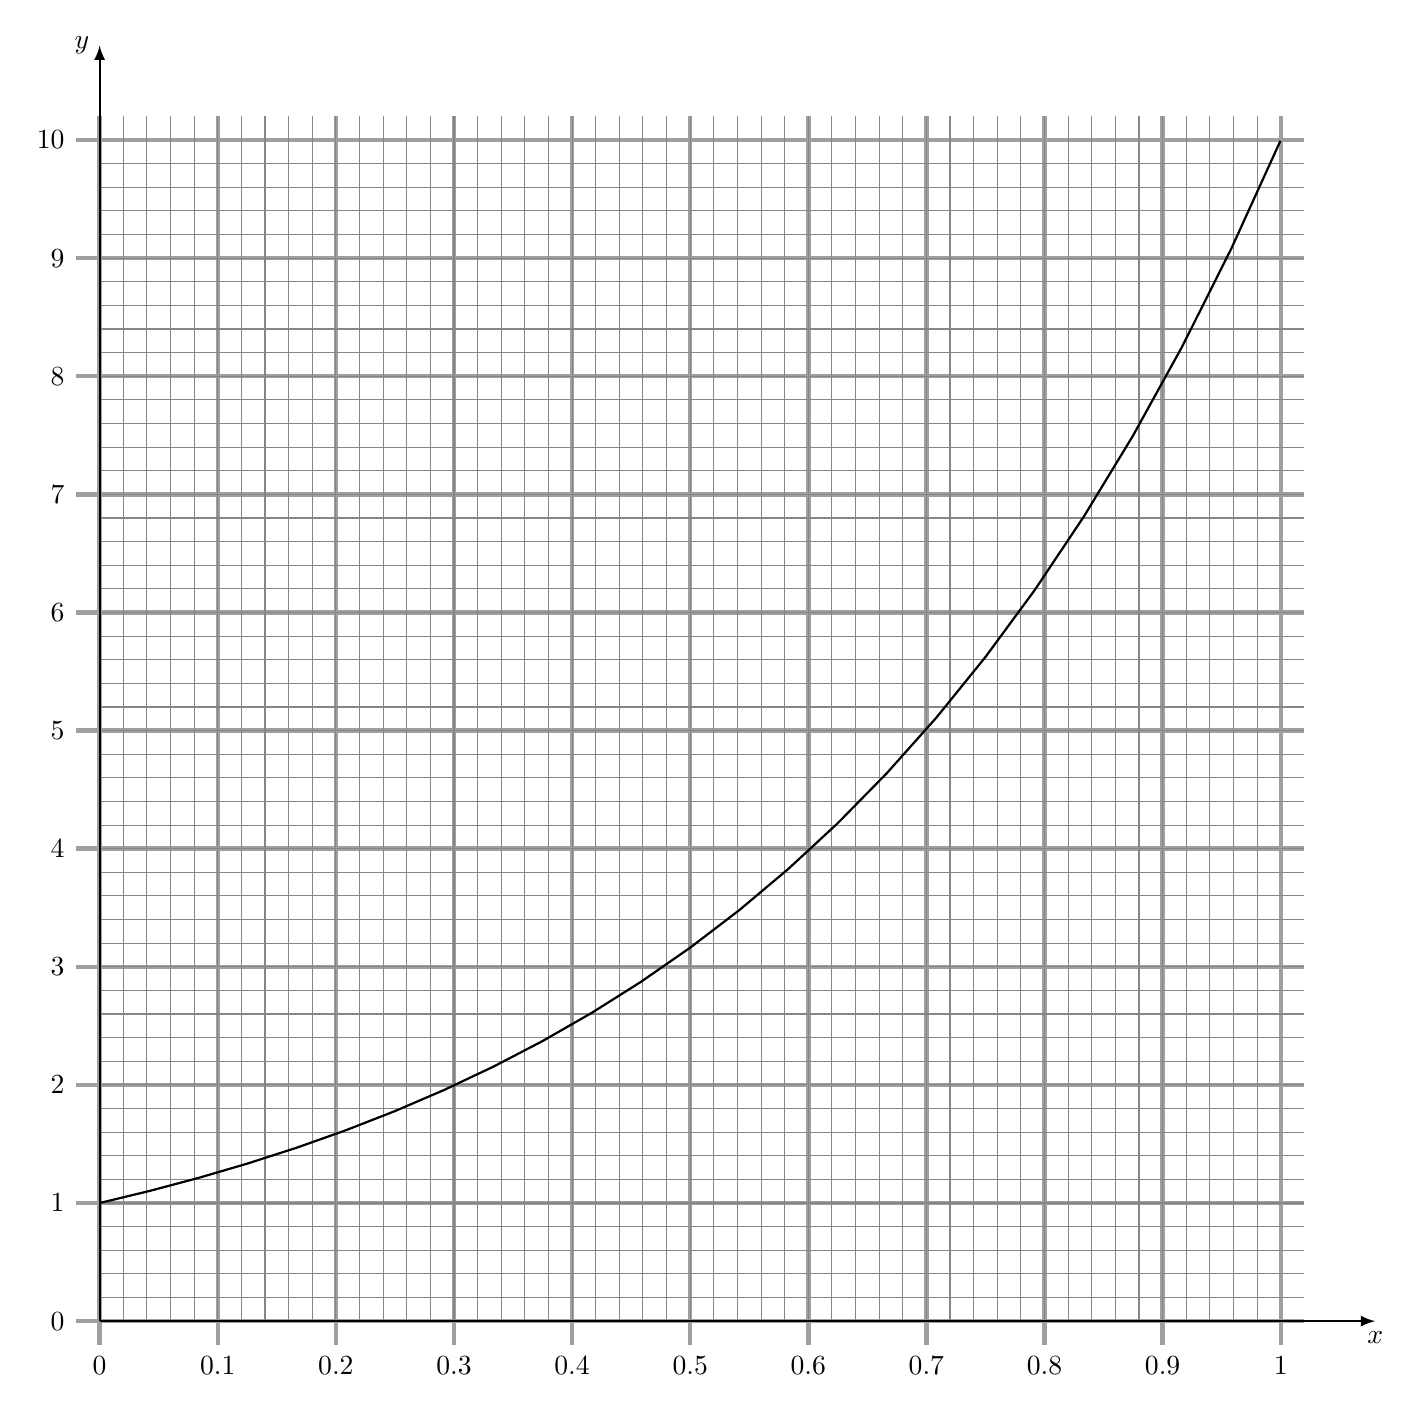
\begin{tikzpicture}[x=150mm,y=15mm,>=latex]
    \foreach \x in {0,0.1,0.2,0.3,0.4,0.5,0.6,0.7,0.8,0.9,1}
    {
      \draw[ultra thick,gray!75] (\x,10.2) -- (\x,-0.2) node[black,below] {$\x$};
    }
    \foreach \y in {0,1,...,10} 
    {
      \draw[ultra thick,gray!75] (1.02,\y) -- (-0.02,\y) node[black,left] {$\y$};
    }
    \foreach \k in {2,4,...,98}
    {
      \draw[thin,gray!95] ({\k/100},10.2) -- ({\k/100},0);
      \draw[thin,gray!95] (1.02,{\k/10}) -- (0,{\k/10});
    }
    %
    \draw[thick,black,->] (0,0) -- (1.08,0) node[below] {$x$};
    \draw[thick,black,->] (0,0) -- (0,10.8) node[left] {$y$};
    \draw[thick,black] plot[domain=0:1] (\x,{10^(\x)});
    % \node[black,fill=white] at (0.21,8.2) {$y=10^x$};
  \end{tikzpicture}
  \bigskip

  {\Large\textbf{Graph of $y=10^{x}$}}
  \vspace*{0.5in}

  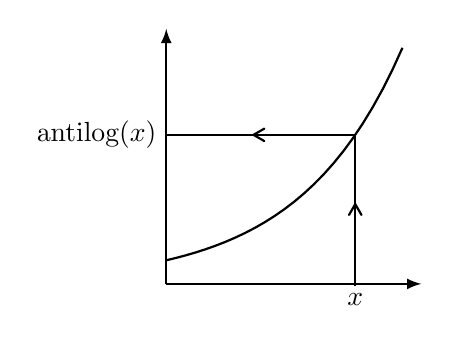
\begin{tikzpicture}[x=30mm,y=3mm,>=latex,baseline=0,decoration={%
      markings,%
      mark=at position 0.55 with {\arrow[double,thick]{angle 60};}}%
      % mark=at position 0.6 with {\arrow{latex};}}%
    ]
    \draw[thick,black,->] (0,0) -- (1.08,0);% node[below] {$x$};
    \draw[thick,black,->] (0,0) -- (0,10.8);% node[left] {$y$};
    \draw[thick,black] plot[domain=0:1] (\x,{10^(\x)});
    \draw[thick,black] (0.8,{ln(0.8)/ln(10)}) -- (0.8,0);
    \node[left] at (0,{10^(0.8)}) {$\mbox{antilog}(x)$};
    \node[below] at (0.8,0) {$x$};
    \draw[thick,black,postaction=decorate] (0.8,{10^(0.8)}) -- (0,{10^(0.8)});
    \draw[thick,black,postaction=decorate] (0.8,0) -- (0.8,{10^(0.8)});
  \end{tikzpicture}
  \hspace*{1.5in}
  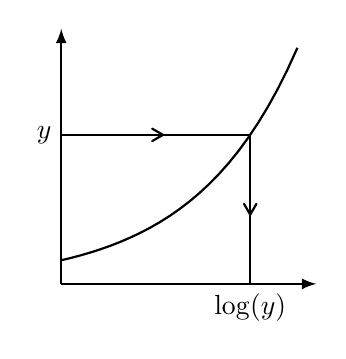
\begin{tikzpicture}[x=30mm,y=3mm,>=latex,baseline=0,decoration={%
      markings,%
      mark=at position 0.55 with {\arrow[double,thick]{angle 60};}}%
      % mark=at position 0.6 with {\arrow{latex};}}%
    ]
    \draw[thick,black,->] (0,0) -- (1.08,0);% node[below] {$x$};
    \draw[thick,black,->] (0,0) -- (0,10.8);% node[left] {$y$};
    \draw[thick,black] plot[domain=0:1] (\x,{10^(\x)});
    \draw[thick,black,postaction=decorate] (0,{10^(0.8)}) -- (0.8,{10^(0.8)});
    \draw[thick,black,postaction=decorate] (0.8,{10^(0.8)}) -- (0.8,0);
    \node[left] at (0,{10^(0.8)}) {$y$};
    \node[below] at (0.8,0) {$\log(y)$};
  \end{tikzpicture}

\end{center}

\end{document}